%%
%% This is file `sample-manuscript.tex',
%% generated with the docstrip utility.
%%
%% The original source files were:
%%
%% samples.dtx  (with options: `manuscript')
%% 
%% IMPORTANT NOTICE:
%% 
%% For the copyright see the source file.
%% 
%% Any modified versions of this file must be renamed
%% with new filenames distinct from sample-manuscript.tex.
%% 
%% For distribution of the original source see the terms
%% for copying and modification in the file samples.dtx.
%% 
%% This generated file may be distributed as long as the
%% original source files, as listed above, are part of the
%% same distribution. (The sources need not necessarily be
%% in the same archive or directory.)
%%
%% Commands for TeXCount
%TC:macro \cite [option:text,text]
%TC:macro \citep [option:text,text]
%TC:macro \citet [option:text,text]
%TC:envir table 0 1
%TC:envir table* 0 1
%TC:envir tabular [ignore] word
%TC:envir displaymath 0 word
%TC:envir math 0 word
%TC:envir comment 0 0
%%
%%
%% The first command in your LaTeX source must be the \documentclass command.
%%%% Small single column format, used for CIE, CSUR, DTRAP, JACM, JDIQ, JEA, JERIC, JETC, PACMCGIT, TAAS, TACCESS, TACO, TALG, TALLIP (formerly TALIP), TCPS, TDSCI, TEAC, TECS, TELO, THRI, TIIS, TIOT, TISSEC, TIST, TKDD, TMIS, TOCE, TOCHI, TOCL, TOCS, TOCT, TODAES, TODS, TOIS, TOIT, TOMACS, TOMM (formerly TOMCCAP), TOMPECS, TOMS, TOPC, TOPLAS, TOPS, TOS, TOSEM, TOSN, TQC, TRETS, TSAS, TSC, TSLP, TWEB.
% \documentclass[acmsmall]{acmart}

%%%% Large single column format, used for IMWUT, JOCCH, PACMPL, POMACS, TAP, PACMHCI
% \documentclass[acmlarge,screen]{acmart}

%%%% Large double column format, used for TOG
% \documentclass[acmtog, authorversion]{acmart}

%%%% Generic manuscript mode, required for submission
%%%% and peer review
\documentclass[manuscript,screen,review]{acmart}
%% Fonts used in the template cannot be substituted; margin 
%% adjustments are not allowed.
%%
%% \BibTeX command to typeset BibTeX logo in the docs
\AtBeginDocument{%
  \providecommand\BibTeX{{%
    \normalfont B\kern-0.5em{\scshape i\kern-0.25em b}\kern-0.8em\TeX}}}

%% Rights management information.  This information is sent to you
%% when you complete the rights form.  These commands have SAMPLE
%% values in them; it is your responsibility as an author to replace
%% the commands and values with those provided to you when you
%% complete the rights form.
\setcopyright{acmcopyright}
\copyrightyear{2018}
\acmYear{2018}
\acmDOI{XXXXXXX.XXXXXXX}

%% These commands are for a PROCEEDINGS abstract or paper.
\acmConference[Conference acronym 'XX]{Make sure to enter the correct
  conference title from your rights confirmation emai}{June 03--05,
  2018}{Woodstock, NY}
%
%  Uncomment \acmBooktitle if th title of the proceedings is different
%  from ``Proceedings of ...''!
%
\acmBooktitle{Woodstock '18: ACM Symposium on Neural Gaze Detection,
 June 03--05, 2018, Woodstock, NY} 
\acmPrice{15.00}
\acmISBN{978-1-4503-XXXX-X/18/06}


%%
%% Submission ID.
%% Use this when submitting an article to a sponsored event. You'll
%% receive a unique submission ID from the organizers
%% of the event, and this ID should be used as the parameter to this command.
%%\acmSubmissionID{123-A56-BU3}

%%
%% For managing citations, it is recommended to use bibliography
%% files in BibTeX format.
%%
%% You can then either use BibTeX with the ACM-Reference-Format style,
%% or BibLaTeX with the acmnumeric or acmauthoryear sytles, that include
%% support for advanced citation of software artefact from the
%% biblatex-software package, also separately available on CTAN.
%%
%% Look at the sample-*-biblatex.tex files for templates showcasing
%% the biblatex styles.
%%

%%
%% The majority of ACM publications use numbered citations and
%% references.  The command \citestyle{authoryear} switches to the
%% "author year" style.
%%
%% If you are preparing content for an event
%% sponsored by ACM SIGGRAPH, you must use the "author year" style of
%% citations and references.
%% Uncommenting
%% the next command will enable that style.
%%\citestyle{acmauthoryear}

%%
%% end of the preamble, start of the body of the document source.
\begin{document}

%%
%% The "title" command has an optional parameter,
%% allowing the author to define a "short title" to be used in page headers.
\title{Personalised nudging using active inference for improving adherence to an exercise plan}

%%
%% The "author" command and its associated commands are used to define
%% the authors and their affiliations.
%% Of note is the shared affiliation of the first two authors, and the
%% "authornote" and "authornotemark" commands
%% used to denote shared contribution to the research.
% \author{Anonymised}
% \authornote{Both authors contributed equally to this research.}
% \email{trovato@corporation.com}
% \orcid{1234-5678-9012}
% \author{G.K.M. Tobin}
% \authornotemark[1]
% \email{webmaster@marysville-ohio.com}
% \affiliation{%
%   \institution{Institute for Clarity in Documentation}
%   \streetaddress{P.O. Box 1212}
%   \city{Dublin}
%   \state{Ohio}
%   \country{USA}
%   \postcode{43017-6221}
% }

% \author{Lars Th{\o}rv{\"a}ld}
% \affiliation{%
%   \institution{The Th{\o}rv{\"a}ld Group}
%   \streetaddress{1 Th{\o}rv{\"a}ld Circle}
%   \city{Hekla}
%   \country{Iceland}}
% \email{larst@affiliation.org}

% \author{Valerie B\'eranger}
% \affiliation{%
%   \institution{Inria Paris-Rocquencourt}
%   \city{Rocquencourt}
%   \country{France}
% }

% \author{Aparna Patel}
% \affiliation{%
%  \institution{Rajiv Gandhi University}
%  \streetaddress{Rono-Hills}
%  \city{Doimukh}
%  \state{Arunachal Pradesh}
%  \country{India}}

% \author{Huifen Chan}
% \affiliation{%
%   \institution{Tsinghua University}
%   \streetaddress{30 Shuangqing Rd}
%   \city{Haidian Qu}
%   \state{Beijing Shi}
%   \country{China}}

% \author{Charles Palmer}
% \affiliation{%
%   \institution{Palmer Research Laboratories}
%   \streetaddress{8600 Datapoint Drive}
%   \city{San Antonio}
%   \state{Texas}
%   \country{USA}
%   \postcode{78229}}
% \email{cpalmer@prl.com}

% \author{John Smith}
% \affiliation{%
%   \institution{The Th{\o}rv{\"a}ld Group}
%   \streetaddress{1 Th{\o}rv{\"a}ld Circle}
%   \city{Hekla}
%   \country{Iceland}}
% \email{jsmith@affiliation.org}

% \author{Julius P. Kumquat}
% \affiliation{%
%   \institution{The Kumquat Consortium}
%   \city{New York}
%   \country{USA}}
% \email{jpkumquat@consortium.net}

%%
%% By default, the full list of authors will be used in the page
%% headers. Often, this list is too long, and will overlap
%% other information printed in the page headers. This command allows
%% the author to define a more concise list
%% of authors' names for this purpose.
\renewcommand{\shortauthors}{Anonymised, et al.}

%%
%% The abstract is a short summary of the work to be presented in the
%% article.
\begin{abstract}
Motivation is often a major obstacle to adherence to an exercise plan.
For instance, poor adherence to rehabilitation programs has been observed,
despite the importance they can have, notably in the treatment of cardiovascular conditions.
In this work, we explore how nudging through personalized incentives
(small monetary rewards spread over the day)
can improve adherence to a daily exercise goal in participants.
For personalizing the incentives, we are using the active inference
framework that allows us to deal with the trade-off between learning
about how the policy concerning the incentives
affects the participant's behavior and helping them meet their objective.
\end{abstract}

%%
%% The code below is generated by the tool at http://dl.acm.org/ccs.cfm.
%% Please copy and paste the code instead of the example below.
%%
% TODO: Generate CODE
\begin{CCSXML}
<ccs2012>
 <concept>
  <concept_id>00000000.0000000.0000000</concept_id>
  <concept_desc>Do Not Use This Code, Generate the Correct Terms for Your Paper</concept_desc>
  <concept_significance>500</concept_significance>
 </concept>
 <concept>
  <concept_id>00000000.00000000.00000000</concept_id>
  <concept_desc>Do Not Use This Code, Generate the Correct Terms for Your Paper</concept_desc>
  <concept_significance>300</concept_significance>
 </concept>
 <concept>
  <concept_id>00000000.00000000.00000000</concept_id>
  <concept_desc>Do Not Use This Code, Generate the Correct Terms for Your Paper</concept_desc>
  <concept_significance>100</concept_significance>
 </concept>
 <concept>
  <concept_id>00000000.00000000.00000000</concept_id>
  <concept_desc>Do Not Use This Code, Generate the Correct Terms for Your Paper</concept_desc>
  <concept_significance>100</concept_significance>
 </concept>
</ccs2012>
\end{CCSXML}

\ccsdesc[500]{Do Not Use This Code~Generate the Correct Terms for Your Paper}
\ccsdesc[300]{Do Not Use This Code~Generate the Correct Terms for Your Paper}
\ccsdesc{Do Not Use This Code~Generate the Correct Terms for Your Paper}
\ccsdesc[100]{Do Not Use This Code~Generate the Correct Terms for Your Paper}

%%
%% Keywords. The author(s) should pick words that accurately describe
%% the work being presented. Separate the keywords with commas.
\keywords{nudging, active inference, model-based} % TODO: keywords

%% A "teaser" image appears between the author and affiliation
%% information and the body of the document, and typically spans the
%% page.
\begin{teaserfigure}
  % 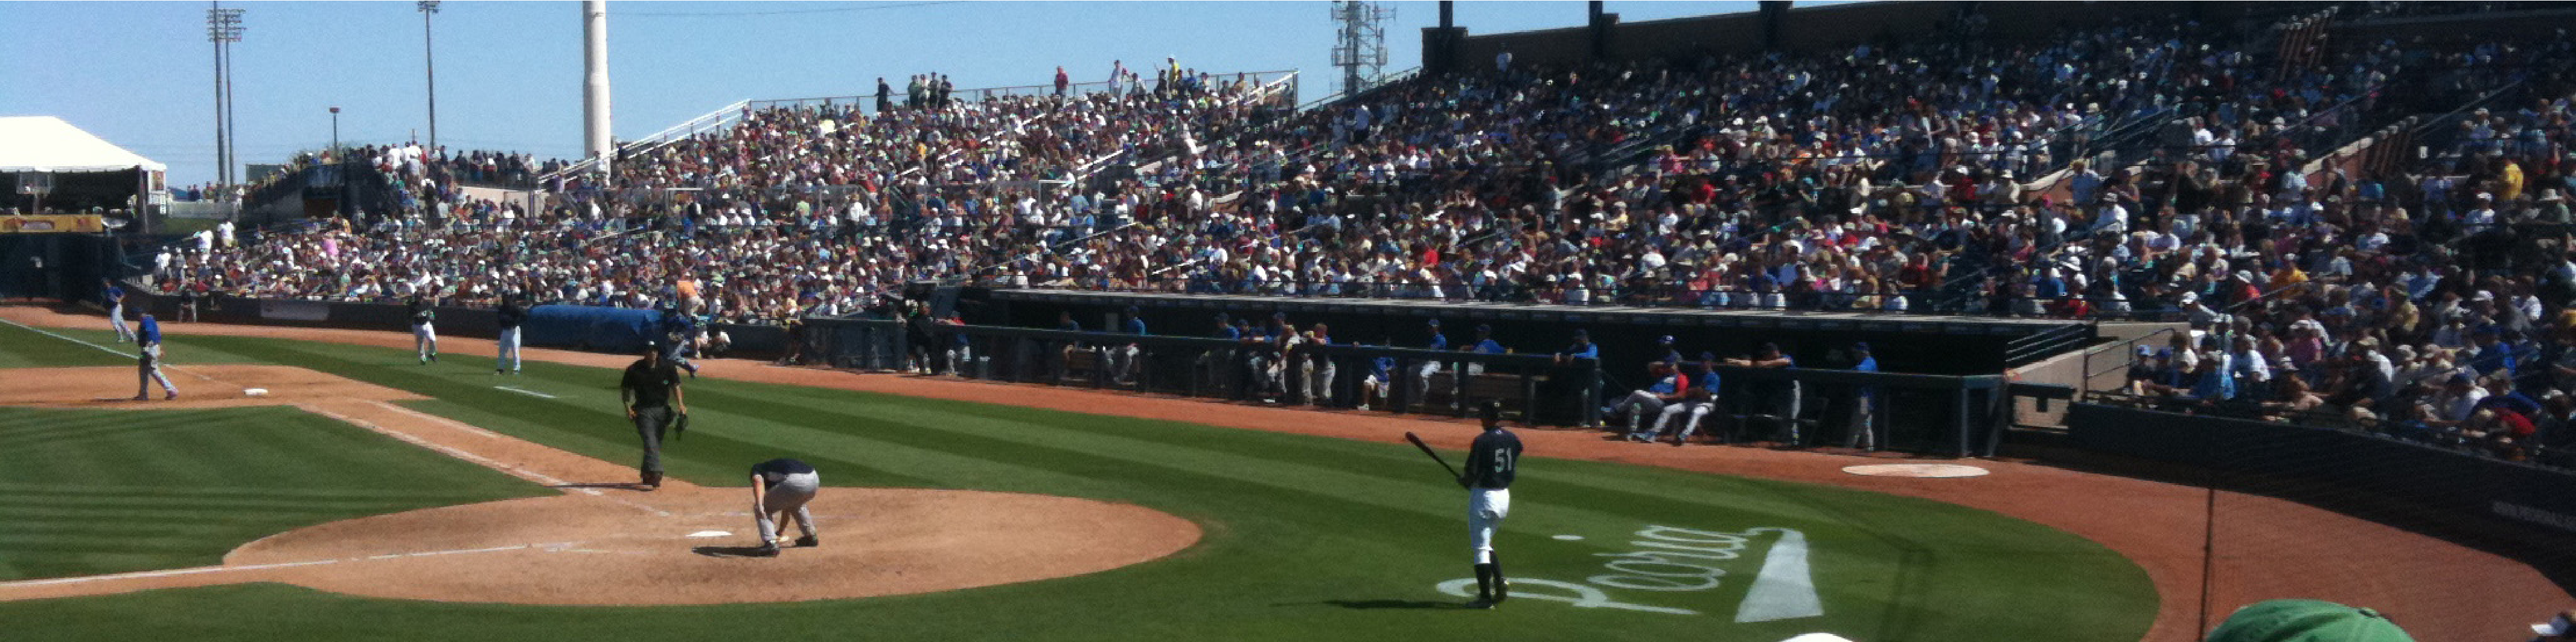
\includegraphics[width=\textwidth]{sampleteaser}
  \caption{}
  \Description{}
  \label{fig:teaser}
\end{teaserfigure}

\received{20 February 2007}
\received[revised]{12 March 2009}
\received[accepted]{5 June 2009}

%%
%% This command processes the author and affiliation and title
%% information and builds the first part of the formatted document.
\maketitle

\section{Introduction}

Adherence to an exercise plan is crucial for maintaining good health and preventing chronic diseases. However,
motivation is often a major obstacle to adherence, even in the context of rehabilitation programs where the stakes
are high \cite{daly2002barriers}. In this work, we explore how such personalized nudging, which is the use of behavioral insights to design interventions that are tailored to an individual’s specific needs and preferences, can improve adherence to a daily exercise goal in participants.

To personalize the incentives (i.e. nudging), we use the active inference framework, which allows us to
balance
learning about how the policy concerning the incentives affects the participant’s behaviour and helping them meet
their objective. Active inference is a mathematical framework that originated in computational neuroscience as a
theory of how the brain implements action, perception, and learning. It has recently been shown to be a promising
approach to the problems of state estimation and control under uncertainty, as well as a foundation for the
construction of goal-driven behaviours in robotics and artificial agents in general. In this work, we would like to
show that it is also a promising approach to the problem of designing personalized nudging interventions.

After presenting the related works, we first give a vision of the computational problem at stake, and then
provide a concrete case of an application where we personalize nudging through small monetary incentives spread over the day to improve adherence to a daily step goal in healthy participants.


\section{Related Work}

There is a growing body of research on the use of personalized nudging to promote healthy behaviours, including exercise.
Personalized nudging refers to the use of behavioural insights to design interventions that are tailored to an individual’s
specific needs and preferences\cite{mills_2022}. This approach has been shown to be effective in promoting a variety
of healthy behaviours, including physical activity\cite{forberger2019nudging}.

One study found that personalized nudging can be used to promote physical activity among older
adults\cite{room2017interventions}. The study used a two-component framework for personalization, which involved
personalizing both the choices being nudged towards (choice personalization) and the method of nudging itself
(delivery personalization). The results showed that personalized nudging was effective in increasing physical activity levels among older adults.

Another study investigated the use of choice architecture techniques to promote physical activity at the population
level \cite{forberger2019nudging}. The study found that while nudging interventions were commonly used to promote
physical activity, most interventions were implemented at the individual level. The authors suggest that there is a need for more research on the use of nudging interventions at the population level.

In addition to personalized nudging, there are other approaches that have been used to promote physical activity. A
pilot program in the UK is exploring the use of financial incentives, such as vouchers and discounts, to encourage
adults to make healthier choices, including increasing physical activity \cite{govuk2021}.
A systematic review found that social support, particularly from family members, is positively associated with
physical activity levels in older adults \cite{lindsay2017association}. Another study found that social support can enable physical activity
uptake and maintenance through encouragement, resources, and companionship \cite{smith2023relationship}.

In the context of improving adherence to an exercise plan, personalized nudging using active inference could be a promising approach. Active inference is a framework for understanding decision-making and behavior that has been applied in various domains. By incorporating individual differences and personalizing the nudges, it may be possible to improve adherence to an exercise plan.

Active inference is based on the free energy principle, which suggests that the brain reduces surprise or uncertainty
 by making predictions based on internal models and updating them using sensory input \cite{mann2022free}. This
 principle integrates  Bayesian inference with active inference, where actions are guided by predictions and sensory feedback refines them.
  It has wide-ranging implications for comprehending brain function, perception, and action
  \cite{bruineberg2018anticipating}. Although Active inference is a mathematical framework that originated in
  computational neuroscience, it has recently been shown to be a promising approach to the problems of
  state-estimation and control under uncertainty, as well as a foundation for the construction of goal-driven
  behaviors in robotics and artificial agents in general\cite{lanillos2021active}. In particular, active inference
  has been used to augment traditional reinforcement learning approaches by furnishing an inherent balance of
  exploration and exploitation, and providing a more flexible conceptualization of
  reward\cite{tschantz2020reinforcement}. Active inference has also been applied to social robotics, where it has
  been shown to have potential in terms of adaptation, generalization, and robustness\cite{da2022active}.

In summary, personalized nudging using active inference could be a powerful tool for improving adherence to an exercise plan. By taking into account individual differences and personalizing the nudges, it may be possible to achieve better outcomes than with traditional nudging approaches.


\section{Personalizing Nudging}

\subsection{Problem Formulation}

We consider two agents interacting with each other: the \textbf{user} and the \textbf{assistant}.
The goal of the assistant is to help the user adhering their objective in terms of physical activity. In this paper, we
 address the problem of the assistant point of view, which is to pick up an intervention $a \in \mathcal{A}$ that will
 help the learner to meet this objective.

We assume that time is discrete. We assume a succession of phases, each of which is a \textit{active phase} or a
\textit{passive phase}. During the active phase, the assistant can take an action $a \in \mathcal{A}$, which is to
propose an intervention to the user. During the passive phase, the assistant cannot take any action.
Each time step, regardless of the phase they are currently in, the assistant observes $o_t \in \mathbb{R}^N$,
the part of the context which can be observed, such as the user behavior or the time of the day. There is also a part
 of the context that the assistant cannot observe,
$z_t \in \mathbb{R}^M$, such as the user intentions or motivation. The part of the context that is not observed is
assumed to be a Markov process, i.e $z_{t+1} \prop p(z_{t+1} \mid z_t, a_t)$. However, we do not assume that this
transition
probability
$p(z, a)$ is known by the assistant. The assistant would need to maintaining a belief $b_t$ over the probability
distribution of transitioning from one state to another, that is $q(p(z_{t+1} \mid z_t, a_t))$.



\subsection{Implementation using Active Inference}

Using the active inference framework,

\begin{equation}
Q^*(\pi) \sim - \sum_{t}^{T} \mathbb E_{Q(o_t, z_t \mid \pi)} \left[\ln Q(z_t \mid \pi) - \ln \tilde p(o_t, z_t) \right]
\end{equation}

\begin{equation}
    = \sum_{t}^{T}  \underbrace{ \mathbb E_{Q(o_t, z_t \mid \pi)} D_{KL}\left[ Q(z_t \mid o_t) || Q(z_t \mid \pi) \right] }_{ \text{epistemic value} }
    + \underbrace{ \mathbb E_{Q(o_t \mid \pi) } \left[ \ln \tilde p(o_t) \right]}_{ \text{pragmatic value} } + \text{const}
\end{equation}

\section{Specific case of application: increasing the daily step count by offering money incentives for completing
challenges}





\section{Simulation Study}

\subsection{Methods}

\subsection{Results}


\section{User Study}

\subsection{Participants}

\subsection{Procedure}

\subsection{Results}

\begin{figure}[h]
  \centering
  \includegraphics[width=\linewidth]{}
  \caption{}
  \Description{}
\end{figure}

% \begin{figure}[h]
%   \centering
%   \includegraphics[width=\linewidth]{}
%   \caption{}
%   \Description{}
% \end{figure}

\section{Discussion}

\section{Conclusion}

%%
%% The acknowledgments section is defined using the "acks" environment
%% (and NOT an unnumbered section). This ensures the proper
%% identification of the section in the article metadata, and the
%% consistent spelling of the heading.
\begin{acks}
We thank all study participants for their time, and our colleagues and the reviewers for their helpful comments.
This work was supported by the Engineering and Physical Sciences Research Council (EPSRC) under grant number BC307829-06 ("Quest").
\end{acks}

%%
%% The next two lines define the bibliography style to be used, and
%% the bibliography file.
\bibliographystyle{ACM-Reference-Format}
\bibliography{biblio}

%%
%% If your work has an appendix, this is the place to put it.
\appendix

\end{document}
\endinput
%%
%% End of file `sample-authordraft.tex'.
